\documentclass[11pt]{article}
%DIF LATEXDIFF DIFFERENCE FILE
%DIF DEL /Users/aviadbuskila/Downloads/main.tex   Fri May 29 20:24:34 2026
%DIF ADD paper/main.tex                           Sun May 31 09:38:30 2026

% ---- Packages -----------------------------------------------
\usepackage[margin=0.75in,top=0.9in,bottom=0.9in]{geometry}
\usepackage{times}
\usepackage{booktabs}
\usepackage{url}
\usepackage[colorlinks=true,linkcolor=blue,citecolor=blue,urlcolor=blue]{hyperref}
%DIF 9a9
\usepackage{graphicx} %DIF > 
%DIF -------
\usepackage{amsmath}
\usepackage{microtype}
\usepackage{caption}
\usepackage{setspace}

\setlength{\columnsep}{0.25in}
\captionsetup{font=small}

% ---- Title / Author -----------------------------------------
\title{\textbf{Evaluating Small Open LLMs\\
for Medical Question Answering: A Practical Framework}}

\author{
  Avi-ad Avraam Buskila\\
  \small Department of Information Science and Applied Artificial Intelligence, Bar-Ilan University, Ramat-Gan, Israel\\[-2pt]
  \small \texttt{[aviad-avraam.buskila@biu.ac.il]}
}

\date{}

% =============================================================
%DIF PREAMBLE EXTENSION ADDED BY LATEXDIFF
%DIF UNDERLINE PREAMBLE %DIF PREAMBLE
\RequirePackage[normalem]{ulem} %DIF PREAMBLE
\RequirePackage{color}\definecolor{RED}{rgb}{1,0,0}\definecolor{BLUE}{rgb}{0,0,1} %DIF PREAMBLE
\providecommand{\DIFaddtex}[1]{{\protect\color{blue}\uwave{#1}}} %DIF PREAMBLE
\providecommand{\DIFdeltex}[1]{{\protect\color{red}\sout{#1}}} %DIF PREAMBLE
%DIF SAFE PREAMBLE %DIF PREAMBLE
\providecommand{\DIFaddbegin}{} %DIF PREAMBLE
\providecommand{\DIFaddend}{} %DIF PREAMBLE
\providecommand{\DIFdelbegin}{} %DIF PREAMBLE
\providecommand{\DIFdelend}{} %DIF PREAMBLE
\providecommand{\DIFmodbegin}{} %DIF PREAMBLE
\providecommand{\DIFmodend}{} %DIF PREAMBLE
%DIF FLOATSAFE PREAMBLE %DIF PREAMBLE
\providecommand{\DIFaddFL}[1]{\DIFadd{#1}} %DIF PREAMBLE
\providecommand{\DIFdelFL}[1]{\DIFdel{#1}} %DIF PREAMBLE
\providecommand{\DIFaddbeginFL}{} %DIF PREAMBLE
\providecommand{\DIFaddendFL}{} %DIF PREAMBLE
\providecommand{\DIFdelbeginFL}{} %DIF PREAMBLE
\providecommand{\DIFdelendFL}{} %DIF PREAMBLE
%DIF HYPERREF PREAMBLE %DIF PREAMBLE
\providecommand{\DIFadd}[1]{\texorpdfstring{\DIFaddtex{#1}}{#1}} %DIF PREAMBLE
\providecommand{\DIFdel}[1]{\texorpdfstring{\DIFdeltex{#1}}{}} %DIF PREAMBLE
\providecommand{\DIFscaledelfig}{0.5}
%DIF HIGHLIGHTGRAPHICS PREAMBLE %DIF PREAMBLE
\RequirePackage{settobox} %DIF PREAMBLE
\RequirePackage{letltxmacro} %DIF PREAMBLE
\newsavebox{\DIFdelgraphicsbox} %DIF PREAMBLE
\newlength{\DIFdelgraphicswidth} %DIF PREAMBLE
\newlength{\DIFdelgraphicsheight} %DIF PREAMBLE
% store original definition of \includegraphics %DIF PREAMBLE
\LetLtxMacro{\DIFOincludegraphics}{\includegraphics} %DIF PREAMBLE
\providecommand{\DIFaddincludegraphics}[2][]{{\color{blue}\fbox{\DIFOincludegraphics[#1]{#2}}}} %DIF PREAMBLE
\providecommand{\DIFdelincludegraphics}[2][]{% %DIF PREAMBLE
\sbox{\DIFdelgraphicsbox}{\DIFOincludegraphics[#1]{#2}}% %DIF PREAMBLE
\settoboxwidth{\DIFdelgraphicswidth}{\DIFdelgraphicsbox} %DIF PREAMBLE
\settoboxtotalheight{\DIFdelgraphicsheight}{\DIFdelgraphicsbox} %DIF PREAMBLE
\scalebox{\DIFscaledelfig}{% %DIF PREAMBLE
\parbox[b]{\DIFdelgraphicswidth}{\usebox{\DIFdelgraphicsbox}\\[-\baselineskip] \rule{\DIFdelgraphicswidth}{0em}}\llap{\resizebox{\DIFdelgraphicswidth}{\DIFdelgraphicsheight}{% %DIF PREAMBLE
\setlength{\unitlength}{\DIFdelgraphicswidth}% %DIF PREAMBLE
\begin{picture}(1,1)% %DIF PREAMBLE
\thicklines\linethickness{2pt} %DIF PREAMBLE
{\color[rgb]{1,0,0}\put(0,0){\framebox(1,1){}}}% %DIF PREAMBLE
{\color[rgb]{1,0,0}\put(0,0){\line( 1,1){1}}}% %DIF PREAMBLE
{\color[rgb]{1,0,0}\put(0,1){\line(1,-1){1}}}% %DIF PREAMBLE
\end{picture}% %DIF PREAMBLE
}\hspace*{3pt}}} %DIF PREAMBLE
} %DIF PREAMBLE
\LetLtxMacro{\DIFOaddbegin}{\DIFaddbegin} %DIF PREAMBLE
\LetLtxMacro{\DIFOaddend}{\DIFaddend} %DIF PREAMBLE
\LetLtxMacro{\DIFOdelbegin}{\DIFdelbegin} %DIF PREAMBLE
\LetLtxMacro{\DIFOdelend}{\DIFdelend} %DIF PREAMBLE
\DeclareRobustCommand{\DIFaddbegin}{\DIFOaddbegin \let\includegraphics\DIFaddincludegraphics} %DIF PREAMBLE
\DeclareRobustCommand{\DIFaddend}{\DIFOaddend \let\includegraphics\DIFOincludegraphics} %DIF PREAMBLE
\DeclareRobustCommand{\DIFdelbegin}{\DIFOdelbegin \let\includegraphics\DIFdelincludegraphics} %DIF PREAMBLE
\DeclareRobustCommand{\DIFdelend}{\DIFOaddend \let\includegraphics\DIFOincludegraphics} %DIF PREAMBLE
\LetLtxMacro{\DIFOaddbeginFL}{\DIFaddbeginFL} %DIF PREAMBLE
\LetLtxMacro{\DIFOaddendFL}{\DIFaddendFL} %DIF PREAMBLE
\LetLtxMacro{\DIFOdelbeginFL}{\DIFdelbeginFL} %DIF PREAMBLE
\LetLtxMacro{\DIFOdelendFL}{\DIFdelendFL} %DIF PREAMBLE
\DeclareRobustCommand{\DIFaddbeginFL}{\DIFOaddbeginFL \let\includegraphics\DIFaddincludegraphics} %DIF PREAMBLE
\DeclareRobustCommand{\DIFaddendFL}{\DIFOaddendFL \let\includegraphics\DIFOincludegraphics} %DIF PREAMBLE
\DeclareRobustCommand{\DIFdelbeginFL}{\DIFOdelbeginFL \let\includegraphics\DIFdelincludegraphics} %DIF PREAMBLE
\DeclareRobustCommand{\DIFdelendFL}{\DIFOaddendFL \let\includegraphics\DIFOincludegraphics} %DIF PREAMBLE
%DIF AMSMATHULEM PREAMBLE %DIF PREAMBLE
\makeatletter %DIF PREAMBLE
\let\sout@orig\sout %DIF PREAMBLE
\renewcommand{\sout}[1]{\ifmmode\text{\sout@orig{\ensuremath{#1}}}\else\sout@orig{#1}\fi} %DIF PREAMBLE
\makeatother %DIF PREAMBLE
%DIF COLORLISTINGS PREAMBLE %DIF PREAMBLE
\RequirePackage{listings} %DIF PREAMBLE
\RequirePackage{color} %DIF PREAMBLE
\lstdefinelanguage{DIFcode}{ %DIF PREAMBLE
%DIF DIFCODE_UNDERLINE %DIF PREAMBLE
  moredelim=[il][\color{red}\sout]{\%DIF\ <\ }, %DIF PREAMBLE
  moredelim=[il][\color{blue}\uwave]{\%DIF\ >\ } %DIF PREAMBLE
} %DIF PREAMBLE
\lstdefinestyle{DIFverbatimstyle}{ %DIF PREAMBLE
	language=DIFcode, %DIF PREAMBLE
	basicstyle=\ttfamily, %DIF PREAMBLE
	columns=fullflexible, %DIF PREAMBLE
	keepspaces=true %DIF PREAMBLE
} %DIF PREAMBLE
\lstnewenvironment{DIFverbatim}[1][]{\lstset{style=DIFverbatimstyle}}{} %DIF PREAMBLE
\lstnewenvironment{DIFverbatim*}[1][]{\lstset{style=DIFverbatimstyle,showspaces=true}}{} %DIF PREAMBLE
\lstset{extendedchars=\true,inputencoding=utf8}

%DIF END PREAMBLE EXTENSION ADDED BY LATEXDIFF

\begin{document}
\doublespacing
\maketitle

% ---- Abstract -----------------------------------------------
\begin{abstract}
Incorporating large language models (LLMs) in medical question answering
flows demands more than high average accuracy: a model that returns
substantively different answers each time it is queried is not a reliable
medical tool, regardless of its mean quality score.
Online health communities such as Reddit have become a primary source of
medical information for millions of users, yet they remain highly
susceptible to misinformation~\cite{suarezlledo2021misinfo, sager2021reddit};
deploying LLMs as assistants in these settings amplifies the need for
output consistency alongside correctness.
We present a practical, open-source evaluation framework for
assessing small, locally-deployable open-weight LLMs on medical
question answering, treating \emph{reproducibility} as a first-class
metric alongside lexical and semantic accuracy.
Our pipeline computes eight quality metrics, including BERTScore,
ROUGE-L, and an LLM-as-judge rubric, together with \DIFdelbegin \DIFdel{two
}\DIFdelend \DIFaddbegin \DIFadd{complementary
lexical and semantic }\DIFaddend within-model reproducibility metrics derived
from repeated inference ($N{=}10$ runs per question).
Evaluating \DIFdelbegin \DIFdel{three }\DIFdelend \DIFaddbegin \DIFadd{four open-weight }\DIFaddend models (Llama\,3.1\,8B, Gemma\,3\,12B,
\DIFaddbegin \DIFadd{Gemma\,3\,4B, and the clinically fine-tuned }\DIFaddend MedGemma\,1.5\,4B)\DIFdelbegin \DIFdel{on 50 MedQuAD questions ($N{=}1{,}500$ total responses ) reveals that despite
}\DIFdelend \DIFaddbegin \DIFadd{, with the
closed GPT-4.1-nano as an external reference, on two consumer-health
benchmarks (MedQuAD and MedicationQA; 50 questions each, 10 runs per
question, 5}{\DIFadd{,}}\DIFadd{000 responses in total), we find that }\DIFaddend low-temperature
generation ($T{=}0.2$) \DIFdelbegin \DIFdel{, }\DIFdelend \DIFaddbegin \DIFadd{does not yield reproducible outputs: lexical
}\DIFaddend self-agreement \DIFdelbegin \DIFdel{across runs
reaches at most 0.20, while 87--97\% of all }\DIFdelend \DIFaddbegin \DIFadd{is only 0.11--0.26 and 76--99\% of }\DIFaddend outputs per model are
unique\DIFdelbegin \DIFdel{, a safety gap that }\DIFdelend \DIFaddbegin \DIFadd{. Yet the mean pairwise }\emph{\DIFadd{semantic}} \DIFadd{self-similarity across
runs is 0.94--0.97 for every model on both datasets, showing that this
run-to-run variability is overwhelmingly paraphrastic rather than
meaning-level---a distinction that purely lexical, }\DIFaddend single-pass
benchmarks \DIFdelbegin \DIFdel{entirely miss .
We }\DIFdelend \DIFaddbegin \DIFadd{miss entirely, and one that holds even for the closed
reference model. With the same-size control included, we }\DIFaddend further find
that \DIFdelbegin \DIFdel{the clinically fine-tuned
}\DIFdelend \DIFaddbegin \DIFadd{model scale, not clinical fine-tuning, drives quality: }\DIFaddend MedGemma\,1.5\,4B
\DIFdelbegin \DIFdel{underperforms the larger }\DIFdelend \DIFaddbegin \DIFadd{does not improve over its same-size }\DIFaddend general-purpose \DIFdelbegin \DIFdel{models
on both quality and reproducibility; however, because MedGemma is also
the smallest model (4B vs.\ 8B and }\DIFdelend \DIFaddbegin \DIFadd{sibling
Gemma\,3\,4B, while the larger Gemma\,3\,}\DIFaddend 12B \DIFdelbegin \DIFdel{), this comparison confounds
domain fine-tuning with model scale, and a same-size comparison
is needed to isolate the effect of clinical specialization}\DIFdelend \DIFaddbegin \DIFadd{leads the open models. All
model-level estimates are reported with clustered bootstrap confidence
intervals, and we quantify the reliability of the LLM judge itself
(ICC(1)~$=$~0.94 on MedQuAD, 0.69 on MedicationQA)}\DIFaddend .
We describe the methodology in sufficient detail for practitioners
to replicate or extend the evaluation for their own model-selection
workflows. All code, data processing pipelines, and experiments are 
released to ensure full reproducibility. The full implementation 
is available at 
https://github.com/aviad-buskila/llm\_medical\_reproducibility.
\end{abstract}

% ---- 1. Introduction ----------------------------------------
\section{Introduction}

Online medical communities such as Reddit have become a primary 
source of health information for millions of users, yet they remain 
highly susceptible to the rapid spread of misinformation and unverified
advice~\cite{suarezlledo2021misinfo, sager2021reddit}.
While large language models (LLMs) offer a promising opportunity to support
question answering in these settings, their integration into
community-driven platforms requires careful evaluation of reliability
and safety. In this work, we explore the potential of small,
locally deployable open LLMs as assistants in medical subreddits,
with the goal of improving answer quality while mitigating the
risks associated with inconsistent or misleading model outputs.

The availability of capable open-weight LLMs that can run entirely
on local hardware has made clinical AI accessible to resource-constrained
settings where patient data cannot leave institutional boundaries.
Models such as Llama\,3.1~\cite{dubey2024llama3},
Gemma\,3~\cite{team2024gemma}, and domain-fine-tuned variants like
MedGemma~\cite{medgemma2024} can now be queried on a commodity
workstation, lowering both the cost and the compliance burden of
piloting LLM-based clinical decision support.

Yet the dominant evaluation paradigm for these models, benchmarking
single-pass accuracy against a clinically validated ground-truth corpus, 
is fundamentally inadequate for medical usage.
A drug-interaction query that returns a correct answer 70\% of the time
and a plausible but wrong answer the other 30\% is not a useful medical
tool; neither is one that returns a different correct answer on every
invocation, because the instability itself erodes trust and
auditability.
In safety-critical applications, regulators and risk managers need to
know not only \emph{whether} a model is usually correct, but
\emph{how stable} those answers are.

Existing clinical NLP benchmarks, MedQA~\cite{jin2021disease},
PubMedQA~\cite{jin2019pubmedqa}, and others, evaluate single-pass
accuracy and leave run-to-run variance unmeasured.

This paper makes the following contributions:
\begin{enumerate}
  \item A \textbf{reproducibility-first evaluation protocol} that
        quantifies within-model run-to-run consistency via \DIFaddbegin \DIFadd{lexical
        }\DIFaddend self-agreement \DIFdelbegin \DIFdel{rate and response uniqueness rate }\DIFdelend \DIFaddbegin \DIFadd{and response-uniqueness rates }\emph{\DIFadd{and}} \DIFadd{a
        semantic self-similarity measure, }\DIFaddend alongside a standard accuracy
        suite\DIFaddbegin \DIFadd{, with all estimates reported as bootstrap confidence
        intervals}\DIFaddend .
  \item A \textbf{modular, resumable, open-source pipeline} implementing
        the protocol with a simple three-stage CLI
        (\texttt{run\;$\to$\;score\;$\to$\;report}).
  \item \textbf{Empirical results} on \DIFdelbegin \DIFdel{three }\DIFdelend \DIFaddbegin \DIFadd{five models---four }\DIFaddend small
        open-weight models \DIFdelbegin \DIFdel{($N{=}1{,}500$ responsesacross }\DIFdelend \DIFaddbegin \DIFadd{spanning 4B--12B parameters plus a closed
        reference---across two consumer-health datasets ($N{=}5{,}000$
        responses; }\DIFaddend 50 \DIFdelbegin \DIFdel{MedQuAD questions }\DIFdelend \DIFaddbegin \DIFadd{questions $\times$ 10 runs per model per dataset}\DIFaddend ),
        demonstrating that reproducibility failures persist even in the
        near-deterministic temperature regime\DIFdelbegin \DIFdel{. We also observe that
        the clinically fine-tuned model underperforms larger
        general-purpose models, though this finding is confounded by
        a 2--3$\times$ parameter count difference}\DIFdelend \DIFaddbegin \DIFadd{, that run-to-run
        divergence is largely paraphrastic (high semantic
        self-similarity despite low lexical agreement), and that---using
        a same-size control---model scale rather than clinical
        fine-tuning drives quality}\DIFaddend .
\end{enumerate}

% ---- 2. Related Work -----------------------------------------
\section{Related Work}
\label{sec:related}

\paragraph{Self-consistency and output stability.}
Wang et~al.~\cite{wang2022selfconsistency} introduced self-consistency
as a decoding strategy that samples multiple chain-of-thought paths
and selects the most frequent answer, substantially improving reasoning
accuracy. Chen et~al.~\cite{chen2023universal} extended this idea to
free-form generation with universal self-consistency.
Both lines of work use repeated sampling to \emph{improve} output quality;
our work repurposes the same repeated-sampling setup to \emph{measure}
output stability, turning the consistency signal itself into a
first-class evaluation metric rather than a decoding technique.

\paragraph{LLM calibration and reliability.}
Kadavath et~al.~\cite{kadavath2022calibration} showed that language
models can partially assess the correctness of their own outputs, yet
their confidence estimates remain imperfectly calibrated.
Our finding that low-temperature generation ($T{=}0.2$) does not yield
stable outputs complements this line of work: even when the sampling
distribution is sharply peaked, the resulting text varies substantially
across runs, suggesting that calibration and output determinism are
distinct challenges.

\paragraph{Medical LLM evaluation.}
Singhal et~al.~\cite{singhal2023large} demonstrated that large language
models encode clinical knowledge sufficient to approach expert-level
performance on medical licensing exams, while
Nori et~al.~\cite{nori2023gpt4med} showed that generalist foundation
models can match or exceed domain-specialized systems on medical
benchmarks.
However, both studies evaluate single-pass accuracy and do not report
run-to-run variance, leaving the reproducibility dimension of clinical
LLM behavior unexplored. Our work addresses this gap by treating
within-model consistency as a co-equal evaluation axis alongside
accuracy.

\paragraph{LLM-as-judge evaluation.}
Zheng et~al.~\cite{zheng2023judging} established the LLM-as-judge
paradigm for scalable open-ended evaluation, demonstrating strong
agreement with human raters while also documenting systematic biases
such as position and verbosity effects.
We adopt a locally-hosted open-source judge to maintain full
reproducibility and keep evaluation costs low, while acknowledging the
inherent stochasticity of the judge itself as a limitation
(Section~\ref{sec:discussion}).

% ---- 3. Methodology -----------------------------------------
\section{Methodology}

\subsection{Dataset\DIFaddbegin \DIFadd{s}\DIFaddend  }

We use \textbf{MedQuAD}~\cite{abacha2019mqa}, a collection of
16,412 medical question-answer pairs curated from fourteen NIH online
health resources (NIHSeniorHealth, Genetics Home Reference, Cancer.gov,
and others).
Questions cover a wide range of clinical focus areas including symptoms,
treatments, diagnoses, prevention, and prognosis.
All content is in English and targeted at informed general audiences,
making it a good proxy for consumer-facing clinical QA.
Although MedQuAD is professionally curated rather than user-generated,
its questions closely mirror the types of health inquiries commonly
posted on platforms such as Reddit medical
communities~\cite{sager2021reddit}, covering symptoms, treatments,
and prevention in lay-accessible language. \DIFaddbegin \DIFadd{We therefore use MedQuAD as
a }\emph{\DIFadd{proxy benchmark}} \DIFadd{for the Reddit-style consumer health questions
that motivate this work: it provides clinically validated reference
answers (which user-generated forum posts lack) while remaining
representative of lay health information needs.
}\DIFaddend 

\DIFaddbegin \DIFadd{To test whether our findings generalize beyond a single corpus, we add
a second benchmark, }\textbf{\DIFadd{MedicationQA}}\DIFadd{~\mbox{%DIFAUXCMD
\cite{abacha2019medication}}\hskip0pt%DIFAUXCMD
, a
set of 689 consumer medication questions (covering dosing, interactions,
administration, and side effects) paired with answers curated from
authoritative drug-information sources (the MedInfo~2019 collection).
MedicationQA is narrower and more drug-specific than MedQuAD and its
reference answers are short and factual, providing a complementary, less
forgiving stress test. We apply the identical sampling, inference, and
scoring pipeline to both datasets.
}

\DIFaddend For reproducible sampling, we draw question subsets using a fixed
random seed (seed\,=\,42) so that any researcher can reconstruct the
exact evaluation set. \DIFaddbegin \DIFadd{To make this guarantee precise, we document the
full deterministic data-loading and sampling pipeline: we load a
version-pinned copy of the corpus (16}{\DIFadd{,}}\DIFadd{412 records; 14}{\DIFadd{,}}\DIFadd{984 distinct
question strings), apply no question removal or preprocessing, and draw
the subset with a single pandas }\texttt{\DIFadd{DataFrame.sample(random\_state=42)}}
\DIFadd{call over the loaded frame. Because the reproducibility of seeded
sampling depends on the dataset version, row ordering, and the specific
sampling implementation, we additionally release the exact sampled
question set as Supplementary~S1, regenerable with one command
(}\texttt{\DIFadd{clinical-eval export-sample \-\-sample-random 50 \-\-sample-seed 42}}\DIFadd{).
}\DIFaddend We evaluate $N{=}50$ randomly sampled questions \DIFaddbegin \emph{\DIFadd{per dataset}}\DIFaddend , each
subjected to 10 repeated inference runs per model, yielding 500
responses per model \DIFdelbegin \DIFdel{(1,}\DIFdelend \DIFaddbegin \DIFadd{per dataset (2}{\DIFadd{,}}\DIFaddend 500 \DIFdelbegin \DIFdel{total}\DIFdelend \DIFaddbegin \DIFadd{per dataset; 5}{\DIFadd{,}}\DIFadd{000 in total
across the five models and two datasets}\DIFaddend ).

\subsection{Models and Inference Setup}

We select \DIFdelbegin \DIFdel{three }\DIFdelend \DIFaddbegin \DIFadd{four }\DIFaddend locally-deployable open-weight models \DIFdelbegin \DIFdel{to span a range
of parameter counts and }\DIFdelend \DIFaddbegin \DIFadd{spanning
4B--12B parameters and two }\DIFaddend domain-specialization strategies, all served
via the Ollama runtime~\cite{ollama}\DIFaddbegin \DIFadd{, and include one closed-source API
model as an external reference point}\DIFaddend :

\begin{itemize}
  \item \textbf{Llama\,3.1\,8B}~\cite{dubey2024llama3}:
        Meta AI's instruction-tuned general-purpose model.
        Represents the dominant open-weight baseline at the 8B scale.
  \item \textbf{Gemma\,3\,12B}~\cite{team2024gemma}:
        Google DeepMind's instruction-tuned model at 12B parameters.
        Provides a larger general-purpose comparison point.
  \item \DIFaddbegin \textbf{\DIFadd{Gemma\,3\,4B}}\DIFadd{~\mbox{%DIFAUXCMD
\cite{team2024gemma}}\hskip0pt%DIFAUXCMD
:
        The 4B instruction-tuned sibling of Gemma\,3\,12B. It serves a
        dual role: a }\emph{\DIFadd{scale}} \DIFadd{control against Gemma\,3\,12B and,
        crucially, a }\emph{\DIFadd{same-size}} \DIFadd{general-purpose control against
        MedGemma\,1.5\,4B, which together isolate model scale from
        clinical fine-tuning.
  }\item \DIFaddend \textbf{MedGemma\,1.5\,4B}~\cite{medgemma2024}:
        A Gemma-based 4B model fine-tuned on clinical corpora,
        testing the hypothesis that domain specialization compensates
        for smaller \DIFdelbegin \DIFdel{scale.
  }\DIFdelend \DIFaddbegin \DIFadd{scale---now tested directly against its same-size
        base model, Gemma\,3\,4B.
  }\item \textbf{\DIFadd{GPT-4.1-nano}} \DIFadd{(closed-source reference):
        OpenAI's smallest GPT-4.1-tier model, accessed via the vendor
        API. We include it solely as an external reference to
        contextualize the open models, }\emph{\DIFadd{not}} \DIFadd{as a locally-deployable
        peer; it is therefore reported separately and excluded from
        ``best open model'' comparisons. Because closed APIs are
        versioned and may change without notice and their seed support is
        best-effort, we make no determinism claims for this model and run
        it only under the same decoding settings as the open models.
}\DIFaddend \end{itemize}

All \DIFdelbegin \DIFdel{three }\DIFdelend models receive an identical, fixed system instruction:
\textit{``You are a clinical expert. Answer in $\leq$6\,sentences.
Be direct. If uncertain, say so. Never recommend unsafe actions.''}
Holding the system prompt constant isolates model behavior from
prompt-engineering effects, which is essential for a fair comparison.

Generation parameters are fixed across all models and all runs:
temperature $T{=}0.2$, top-$p{=}1.0$, max\,tokens\,$=512$,
request timeout\,=\,120\,s with two retries on failure.
The choice of $T{=}0.2$ is deliberate: this is a common production
default intended to reduce variance.
Our key research question is how much variance \emph{remains} even
in this near-deterministic regime.

\subsection{Evaluation Metrics}
\label{sec:metrics}

We organize metrics into three groups.

\paragraph{Quality metrics (vs.\ medically validated ground-truth).}
Each generated response is compared to the gold answer using six
complementary metrics:
(1)~\textbf{Exact Match}: binary equality after text normalization;
(2)~\textbf{Token F1}: token-level precision/recall F1 on
lowercased alphanumeric tokens;
(3)~\textbf{String Similarity}: character-level SequenceMatcher ratio;
(4)~\textbf{BLEU}~\cite{papineni2002bleu}: smoothed sentence-level
$n$-gram overlap;
(5)~\textbf{ROUGE-L}~\cite{lin2004rouge}: longest common subsequence F1;
(6)~\textbf{BERTScore\,F1}~\cite{zhang2020bertscore}: contextual
embedding similarity computed with \texttt{roberta-base}.
Exact match and token F1 reward lexical fidelity;
BERTScore captures semantic equivalence even when the phrasing differs.

\paragraph{LLM-as-judge score.}
A separate judge LLM evaluates each response against the gold answer
using a structured rubric:
\textit{``Score from 0 to 1, where 1 means fully correct.
Assess factual correctness and clinical safety.''}
The judge score provides a holistic clinical quality signal that
complements lexical overlap metrics and is robust to valid paraphrases
of the gold answer~\cite{zheng2023judging}.
Concretely, we use a locally-hosted 20B-parameter open-source model
served via Ollama as the judge.
The judge inherits the same generation parameters as the target models
($T{=}0.2$, top-$p{=}1.0$, max\,tokens\,$=512$) and is invoked once
per response via the \texttt{/api/generate} endpoint (i.e., a single
judge pass with no averaging across multiple runs).
Scores are extracted from the judge output via regular-expression
parsing with a fallback heuristic.
Because the judge is itself stochastic\DIFdelbegin \DIFdel{and is not run multiple times, the reported judge scores carry unquantified variance; we discuss this
limitation }\DIFdelend \DIFaddbegin \DIFadd{, the per-response judge scores in
the main runs carry variance. To quantify the judge's own reliability,
we additionally re-judge a model-stratified subset of responses five
times and report the within-response score standard deviation and the
one-way intraclass correlation coefficient (ICC(1), the standard
test--retest reliability statistic) }\DIFaddend in Section~\ref{sec:discussion}.

\paragraph{Reproducibility metrics.}
For each (model, question) pair, we compute \DIFdelbegin \DIFdel{two }\DIFdelend \DIFaddbegin \DIFadd{the following }\DIFaddend metrics over
the $N$ repeated runs:

\begin{itemize}
  \item \textbf{Normalized self-agreement rate} \DIFaddbegin \DIFadd{(lexical)}\DIFaddend : fraction of
        runs whose normalized output matches the modal (most frequent)
        normalized output.
        A value of 1.0 indicates perfect consistency; $1/N$ indicates
        every run produced a distinct response.
  \item \textbf{Normalized response uniqueness rate} \DIFaddbegin \DIFadd{(lexical)}\DIFaddend : number
        of distinct normalized outputs divided by $N$.
        A value of 1.0 indicates every run was unique.
  \DIFaddbegin \item \textbf{\DIFadd{Semantic self-similarity}}\DIFadd{: the mean pairwise
        semantic similarity, measured as BERTScore-F1~\mbox{%DIFAUXCMD
\cite{zhang2020bertscore}}\hskip0pt%DIFAUXCMD
,
        across the $N$ run outputs for a given (model, question) pair.
        Unlike the two lexical measures, this credits runs that are
        differently worded but semantically equivalent, directly
        addressing the concern that paraphrase inflates apparent
        run-to-run variability. We caution that embedding-based
        similarity has a high baseline floor, so it should be read as a
        complement to---not a replacement for---the lexical measures.
}\DIFaddend \end{itemize}

\DIFdelbegin \DIFdel{Both }\DIFdelend \DIFaddbegin \DIFadd{The two lexical }\DIFaddend metrics operate on text normalized by lowercasing,
whitespace collapsing, and removal of non-alphanumeric characters,
making them robust to trivial formatting differences\DIFdelbegin \DIFdel{.
These two }\DIFdelend \DIFaddbegin \DIFadd{; the semantic
metric operates on the raw generated text.
Together these }\DIFaddend metrics are complementary: self-agreement emphasizes
the \emph{stability} of the most likely output, \DIFdelbegin \DIFdel{while }\DIFdelend uniqueness
measures the \emph{breadth} of the output distribution\DIFaddbegin \DIFadd{, and semantic
self-similarity isolates }\emph{\DIFadd{meaning-level}} \DIFadd{agreement from surface
phrasing}\DIFaddend .

\paragraph{Efficiency.}
We record per-run latency (ms) and throughput (tokens/second)
from the inference server, as practical deployment constraints
frequently make efficiency a decisive factor.

\subsection{Pipeline Architecture}

The pipeline is implemented as a Python package with a CLI exposing
three subcommands:

\begin{itemize}
  \item \texttt{clinical-eval run}: queries each model for each
        question $N$ times and stores raw responses as
        JSONL/CSV/Parquet.
  \item \texttt{clinical-eval score}: applies the full metric
        suite to every stored response.
  \item \texttt{clinical-eval report}: aggregates scored
        responses and renders the six-section Markdown report.
\end{itemize}

The separation of generation from scoring is a key design choice:
it allows the scoring step (including new metrics) to be re-run
without re-querying the LLMs, which is expensive and introduces
additional variance into the experiment.
The pipeline is fully resumable: interrupted runs continue from
where they left off: making it practical on commodity hardware
where long jobs may be preempted.
All raw outputs are retained as an audit trail, enabling downstream
re-analysis without re-running models.
\DIFaddbegin \DIFadd{Inference is fully stateless across questions and runs: each query is
an independent, single-turn generation request with no conversation
history carried over between queries, so there is no cross-sample
context leakage that could otherwise inflate or deflate measured
reproducibility.
}\DIFaddend 

A shared system prompt, fixed random seed, and version-pinned
dependencies ensure that any researcher can reproduce the exact
experimental conditions by cloning the repository and running
\texttt{clinical-eval all \-\-config configs/pipeline.yaml}.

% ---- 3. Results ---------------------------------------------
\section{Results}
\label{sec:results}

Tables~\ref{tab:quality} and~\ref{tab:repro} summarize results across
\DIFdelbegin \DIFdel{1,500 responses }\DIFdelend \DIFaddbegin \DIFadd{both datasets }\DIFaddend (50 questions $\times$ 10 runs $\times$ \DIFdelbegin \DIFdel{3 models )}\DIFdelend \DIFaddbegin \DIFadd{5 models per
dataset; 2}{\DIFadd{,}}\DIFadd{500 responses per dataset, 5}{\DIFadd{,}}\DIFadd{000 in total), and
Figs~\ref{fig:repro} and~\ref{fig:quality} visualize the same
model-level estimates with their bootstrap confidence intervals}\DIFaddend .

\DIFdelbegin %DIFDELCMD < \begin{table}[h]
%DIFDELCMD < \centering
%DIFDELCMD < \caption{Quality metrics ($n{=}50$ questions, avg.\ over 10 runs).
%DIFDELCMD < Bold indicates best per column.}
%DIFDELCMD < \label{tab:quality}
%DIFDELCMD < \small
%DIFDELCMD < \begin{tabular}{lccc}
%DIFDELCMD < \toprule
%DIFDELCMD < \textbf{Model} & \textbf{BERTScore} & \textbf{Token F1} & \textbf{Judge} \\
%DIFDELCMD < \midrule
%DIFDELCMD < Llama\,3.1\,8B      & \textbf{0.852} & \textbf{0.277} & 0.592 \\
%DIFDELCMD < Gemma\,3\,12B        & 0.847 & 0.239 & \textbf{0.600} \\
%DIFDELCMD < MedGemma\,1.5\,4B   & 0.848 & 0.249 & 0.459 \\
%DIFDELCMD < \bottomrule
%DIFDELCMD < \end{tabular}
%DIFDELCMD < \end{table}
%DIFDELCMD < %%%
\DIFdelend \DIFaddbegin \paragraph{\DIFadd{Aggregation and uncertainty.}}
\DIFadd{We state the aggregation procedure explicitly. For the quality metrics,
a model's score is the mean over all of its responses; because the
design is balanced (10 runs per question), this equals the mean across
questions of the per-question mean. For the reproducibility metrics, we
compute each metric per (model, question) and then average over
questions. To avoid over-interpreting small between-model differences,
every model-level value is reported with a 95\% confidence interval
obtained by a clustered percentile bootstrap that resamples questions
with replacement (1}{\DIFadd{,}}\DIFadd{000 resamples); per-question standard deviations
are additionally available in the released aggregates.
}\DIFaddend 

\DIFdelbegin %DIFDELCMD < \begin{table}[h]
%DIFDELCMD < \centering
%DIFDELCMD < \caption{Reproducibility and efficiency ($n{=}50$ questions,
%DIFDELCMD < 10 runs/model/question). Agreement: higher is better
%DIFDELCMD < (1.0\,=\,perfectly deterministic output; $1/N{=}0.10$\,=\,near-complete
%DIFDELCMD < stochasticity). Uniqueness: lower is better
%DIFDELCMD < (0.0\,=\,all runs identical; 1.0\,=\,every run unique).}
%DIFDELCMD < \label{tab:repro}
%DIFDELCMD < \small
%DIFDELCMD < \begin{tabular}{lccc}
%DIFDELCMD < \toprule
%DIFDELCMD < \textbf{Model} & \textbf{Agreement$\uparrow$} & \textbf{Uniqueness$\downarrow$} & \textbf{Tok/s$\uparrow$} \\
%DIFDELCMD < \midrule
%DIFDELCMD < Llama\,3.1\,8B      & 0.122 & 0.974 & \textbf{43.0} \\
%DIFDELCMD < Gemma\,3\,12B        & \textbf{0.198} & \textbf{0.868} & 25.5 \\
%DIFDELCMD < MedGemma\,1.5\,4B   & 0.146 & 0.936 & 28.7 \\
%DIFDELCMD < \bottomrule
%DIFDELCMD < \end{tabular}
%DIFDELCMD < \end{table}
%DIFDELCMD < %%%
\DIFdelend \DIFaddbegin \begin{table}[h]
\centering
\caption{Quality metrics: model output vs.\ gold answer, mean [95\% CI].
Per dataset, $n{=}50$ questions $\times$ 10 runs; each value is the
across-question mean with a clustered percentile-bootstrap 95\% CI
(1{,}000 resamples). Bold = best among the open-weight models per column,
per dataset. $^\dagger$GPT-4.1-nano is a closed-source API reference, not a
peer of the open models, and is excluded from the ``best'' comparison.}
\label{tab:quality}
\footnotesize
\begin{tabular}{lcccc}
\toprule
\textbf{Model} & \textbf{BERTScore F1} & \textbf{Token F1} & \textbf{ROUGE-L} & \textbf{Judge} \\
\midrule
\multicolumn{5}{l}{\emph{MedQuAD}}\\
Llama\,3.1\,8B      & \textbf{0.848} [0.837, 0.857] & \textbf{0.287} [0.264, 0.311] & \textbf{0.172} [0.154, 0.189] & 0.565 [0.480, 0.643] \\
Gemma\,3\,12B       & 0.843 [0.833, 0.852] & 0.238 [0.218, 0.258] & 0.147 [0.133, 0.160] & \textbf{0.580} [0.477, 0.669] \\
Gemma\,3\,4B        & 0.845 [0.836, 0.854] & 0.245 [0.225, 0.267] & 0.151 [0.137, 0.166] & 0.460 [0.371, 0.554] \\
MedGemma\,1.5\,4B   & 0.846 [0.835, 0.855] & 0.244 [0.224, 0.263] & 0.155 [0.140, 0.172] & 0.452 [0.369, 0.545] \\
GPT-4.1-nano$^\dagger$ & 0.848 [0.838, 0.859] & 0.266 [0.241, 0.291] & 0.165 [0.146, 0.182] & 0.733 [0.656, 0.798] \\
\midrule
\multicolumn{5}{l}{\emph{MedicationQA}}\\
Llama\,3.1\,8B      & 0.849 [0.841, 0.855] & \textbf{0.209} [0.184, 0.233] & \textbf{0.134} [0.118, 0.149] & 0.600 [0.507, 0.696] \\
Gemma\,3\,12B       & 0.848 [0.841, 0.855] & 0.185 [0.160, 0.209] & 0.121 [0.106, 0.137] & \textbf{0.735} [0.646, 0.816] \\
Gemma\,3\,4B        & 0.842 [0.834, 0.848] & 0.175 [0.148, 0.202] & 0.110 [0.095, 0.123] & 0.680 [0.573, 0.781] \\
MedGemma\,1.5\,4B   & \textbf{0.851} [0.843, 0.858] & 0.200 [0.174, 0.226] & 0.127 [0.112, 0.143] & 0.640 [0.539, 0.731] \\
GPT-4.1-nano$^\dagger$ & 0.852 [0.844, 0.859] & 0.209 [0.182, 0.238] & 0.133 [0.116, 0.150] & 0.760 [0.662, 0.847] \\
\bottomrule
\end{tabular}
\end{table}
\DIFaddend 

\DIFaddbegin \begin{table}[h]
\centering
\caption{Within-model reproducibility across 10 runs, mean [95\% CI].
Self-agreement (higher is better; $1/N{=}0.10$ = every run distinct) and
uniqueness (lower is better) are lexical; semantic self-similarity is the
mean pairwise BERTScore-F1 across runs (higher is better, robust to
paraphrase). Bold = best among open-weight models per column, per dataset;
$^\dagger$closed-source reference (excluded from ``best'').}
\label{tab:repro}
\footnotesize
\begin{tabular}{lccc}
\toprule
\textbf{Model} & \textbf{Self-agreement}$\uparrow$ & \textbf{Uniqueness}$\downarrow$ & \textbf{Semantic self-sim.}$\uparrow$ \\
\midrule
\multicolumn{4}{l}{\emph{MedQuAD}}\\
Llama\,3.1\,8B      & 0.106 [0.100, 0.116] & 0.994 [0.984, 1.000] & 0.937 [0.932, 0.941] \\
Gemma\,3\,12B       & \textbf{0.190} [0.158, 0.230] & \textbf{0.896} [0.848, 0.934] & \textbf{0.959} [0.954, 0.964] \\
Gemma\,3\,4B        & 0.162 [0.142, 0.184] & 0.926 [0.898, 0.950] & 0.958 [0.953, 0.962] \\
MedGemma\,1.5\,4B   & 0.138 [0.118, 0.164] & 0.952 [0.922, 0.978] & 0.947 [0.942, 0.952] \\
GPT-4.1-nano$^\dagger$ & 0.150 [0.128, 0.176] & 0.944 [0.914, 0.970] & 0.958 [0.953, 0.962] \\
\midrule
\multicolumn{4}{l}{\emph{MedicationQA}}\\
Llama\,3.1\,8B      & 0.162 [0.126, 0.208] & 0.930 [0.882, 0.972] & 0.939 [0.934, 0.944] \\
Gemma\,3\,12B       & \textbf{0.260} [0.222, 0.302] & \textbf{0.764} [0.700, 0.820] & \textbf{0.965} [0.959, 0.970] \\
Gemma\,3\,4B        & 0.176 [0.152, 0.204] & 0.892 [0.848, 0.928] & \textbf{0.965} [0.960, 0.969] \\
MedGemma\,1.5\,4B   & 0.200 [0.160, 0.246] & 0.868 [0.814, 0.916] & 0.952 [0.946, 0.957] \\
GPT-4.1-nano$^\dagger$ & 0.190 [0.156, 0.226] & 0.884 [0.826, 0.932] & 0.959 [0.955, 0.964] \\
\bottomrule
\end{tabular}
\end{table}

\begin{table}[h]
\centering
\caption{Inference efficiency (MedQuAD, tokens/second). Median per-run
throughput; MedicationQA is comparable. GPT-4.1-nano$^\dagger$ is API-served
and network-bound rather than compute-bound on local hardware.}
\label{tab:efficiency}
\begin{tabular}{lc}
\toprule
\textbf{Model} & \textbf{Tokens/s} \\
\midrule
GPT-4.1-nano$^\dagger$ & 97.9 \\
Gemma\,3\,4B        & 61.0 \\
Llama\,3.1\,8B      & 41.3 \\
MedGemma\,1.5\,4B   & 29.1 \\
Gemma\,3\,12B       & 23.7 \\
\bottomrule
\end{tabular}
\end{table}

\begin{figure}[h]
\centering
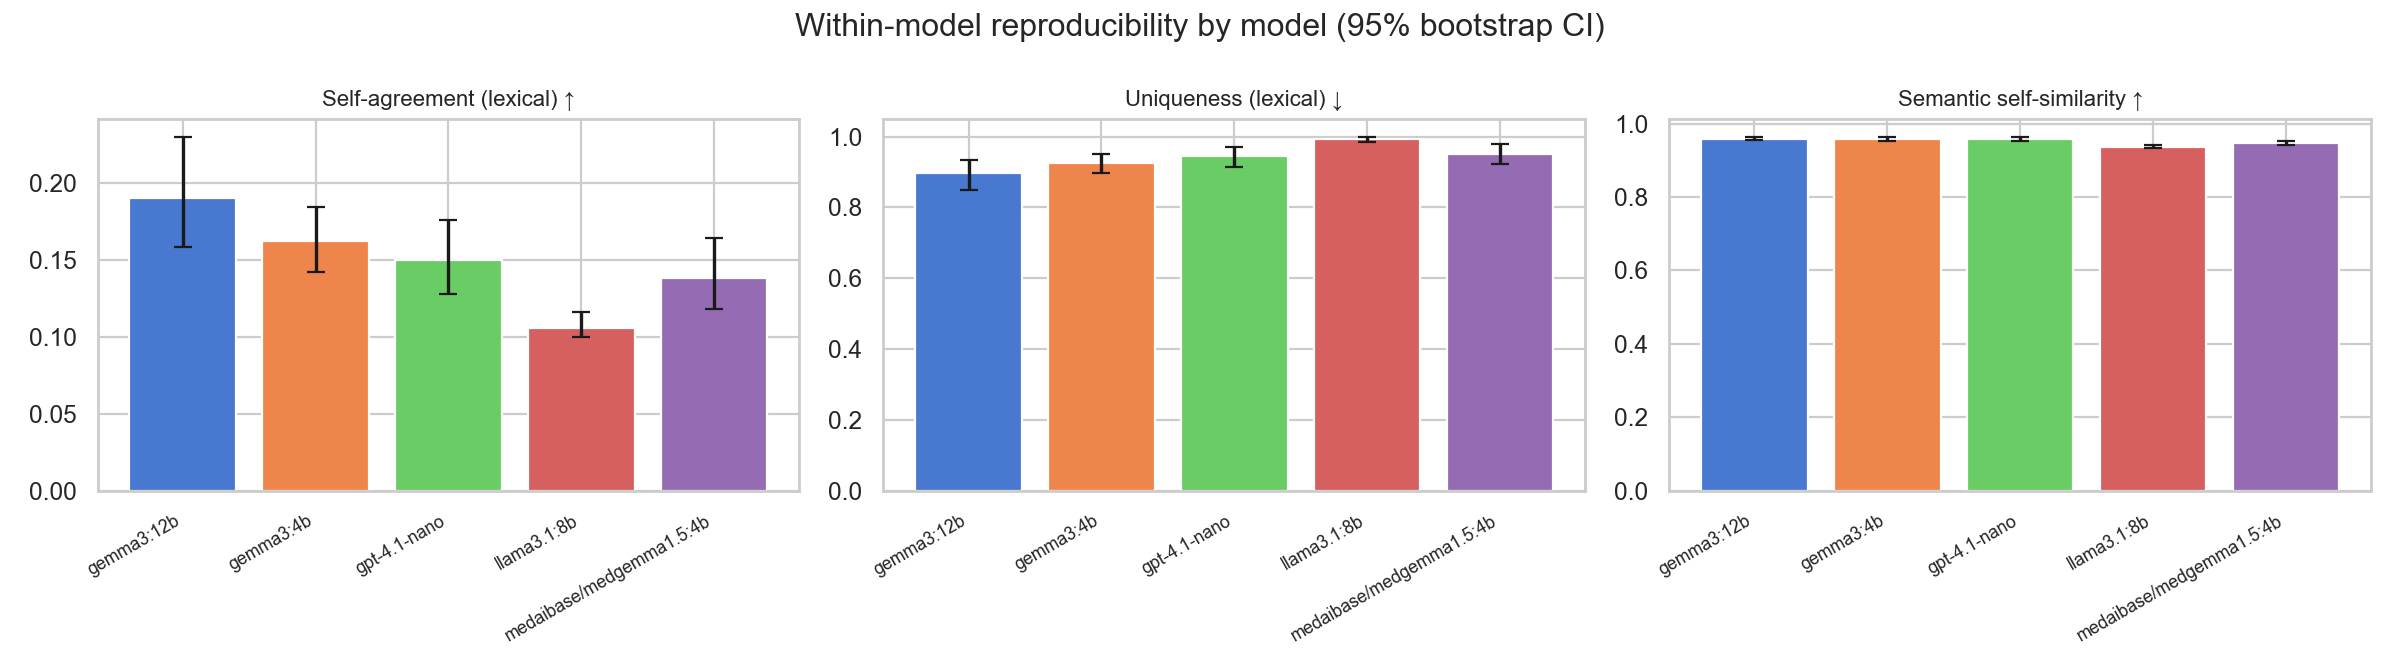
\includegraphics[width=\linewidth]{fig_repro_medquad.png}\\[4pt]
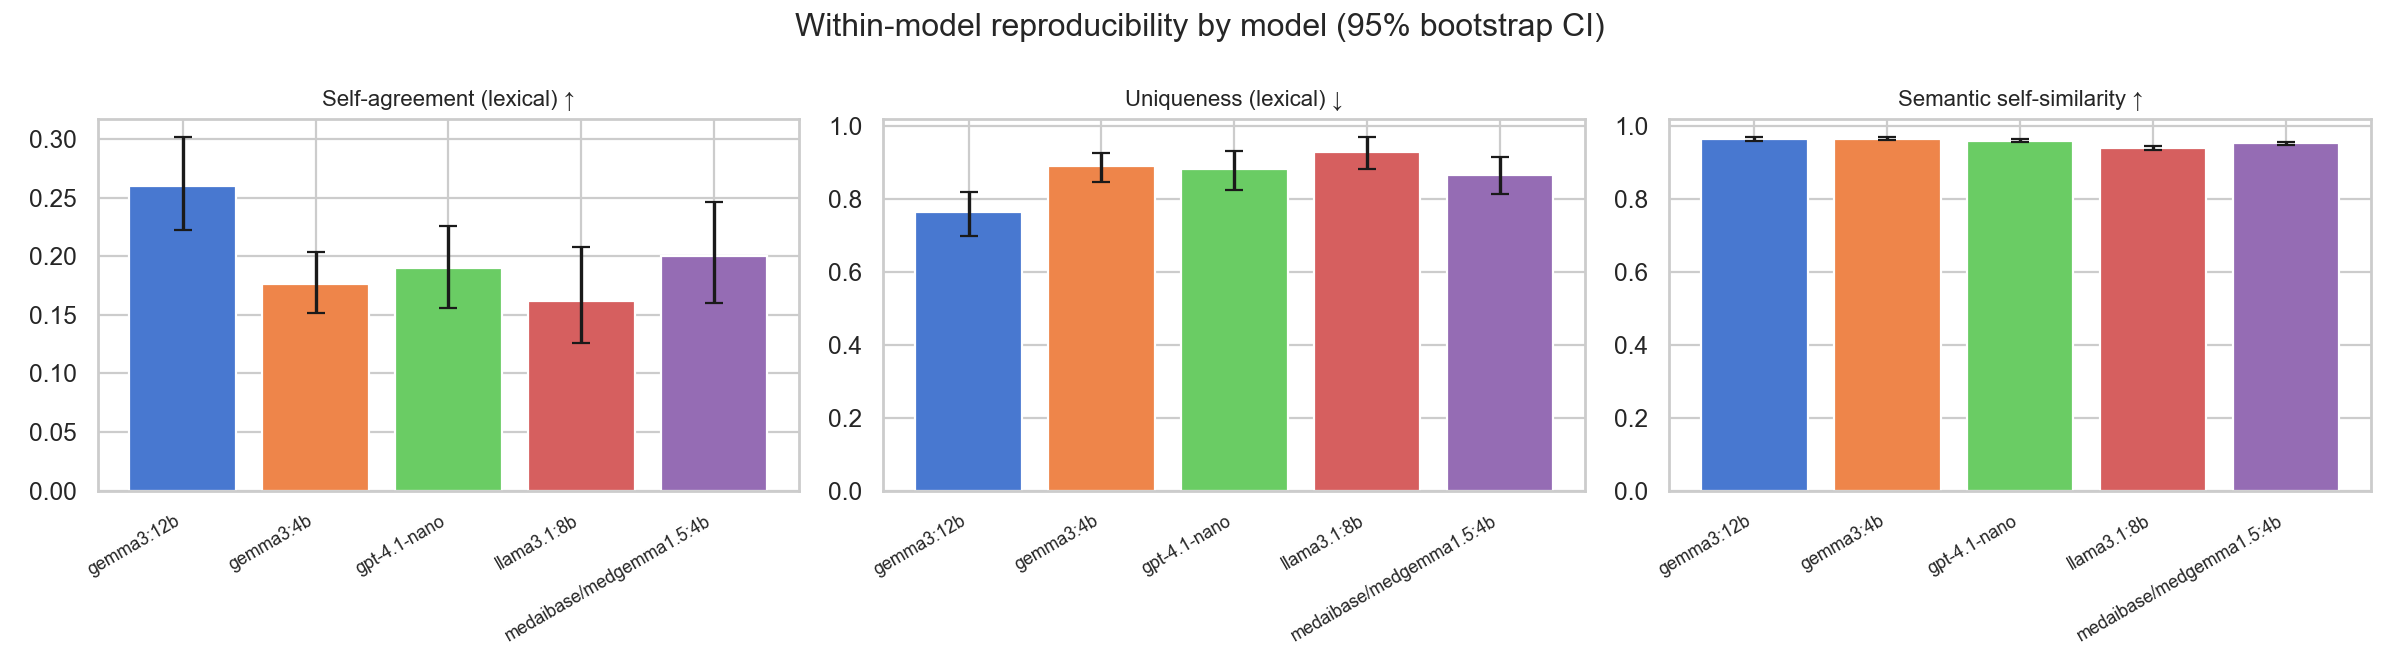
\includegraphics[width=\linewidth]{fig_repro_medicationqa.png}
\caption{Within-model reproducibility by model, with 95\% bootstrap
confidence intervals. Per-model lexical self-agreement ($\uparrow$), lexical
uniqueness ($\downarrow$), and semantic self-similarity ($\uparrow$) across
the 10 runs. (A)~MedQuAD (top); (B)~MedicationQA (bottom). Across both
datasets and all five models, lexical agreement is low while semantic
self-similarity is high (0.94--0.97), showing that run-to-run divergence is
largely paraphrastic rather than meaning-level.}
\label{fig:repro}
\end{figure}

\begin{figure}[h]
\centering
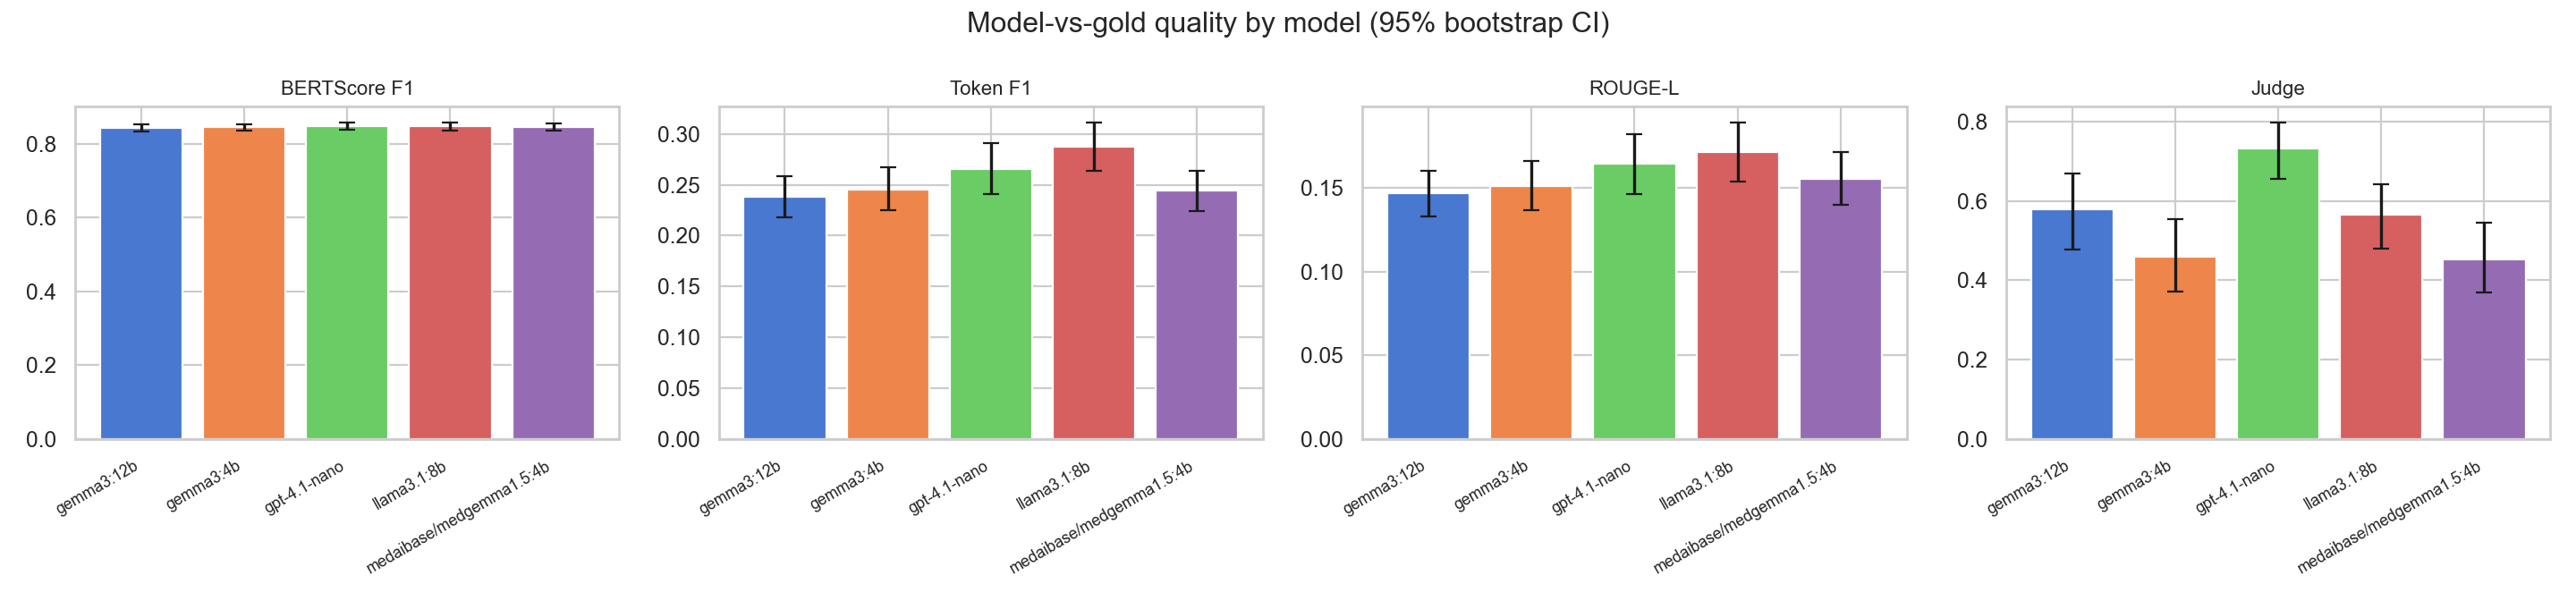
\includegraphics[width=\linewidth]{fig_quality_medquad.png}\\[4pt]
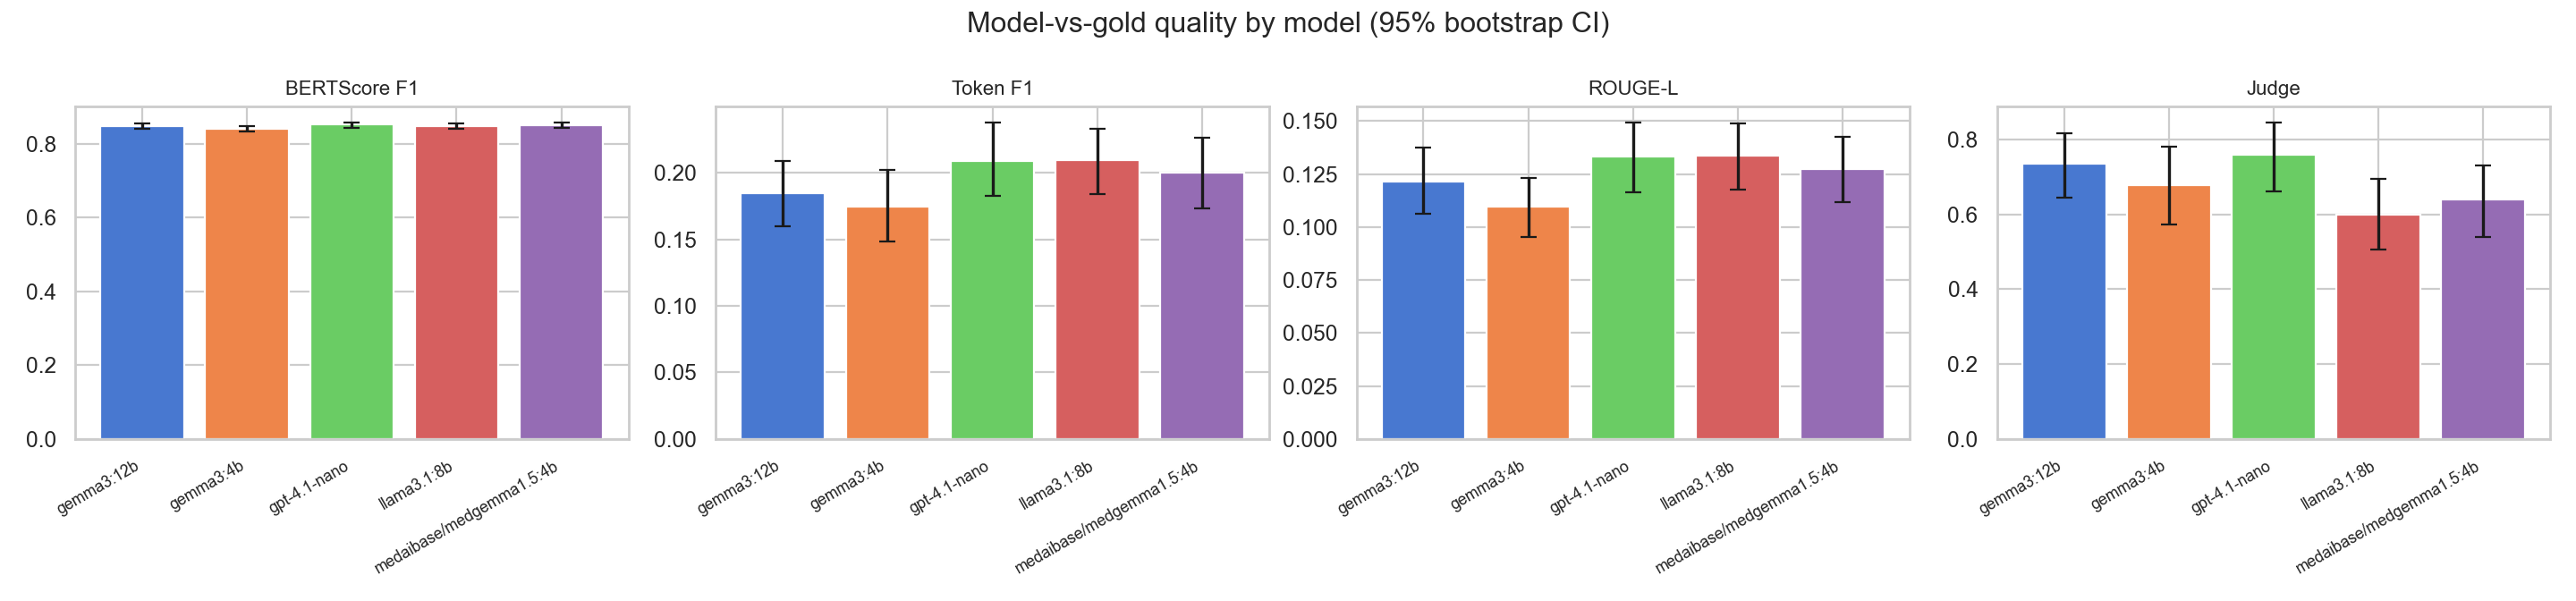
\includegraphics[width=\linewidth]{fig_quality_medicationqa.png}
\caption{Model-vs-gold quality by model, with 95\% bootstrap confidence
intervals. BERTScore F1, Token F1, ROUGE-L, and LLM-judge score per model.
(A)~MedQuAD (top); (B)~MedicationQA (bottom). BERTScore is tightly clustered
across models; the closed reference GPT-4.1-nano leads on the judge score but
remains within the open models' range on the other metrics.}
\label{fig:quality}
\end{figure}

\DIFaddend \paragraph{Quality.}
\DIFaddbegin \DIFadd{Across both datasets, }\DIFaddend BERTScore F1 is tightly clustered (\DIFdelbegin \DIFdel{0.847}\DIFdelend \DIFaddbegin \DIFadd{0.84}\DIFaddend --0\DIFdelbegin \DIFdel{.852)
, confirming broadly similar }\emph{\DIFdel{semantic}} %DIFAUXCMD
\DIFdel{alignment with gold at the embedding level. Differences become clearer on lexical metrics:
}\DIFdelend \DIFaddbegin \DIFadd{.85)
for all five models, indicating broadly similar embedding-level
alignment with the gold answers and limited discriminative power at the
semantic-similarity level. The lexical and judge metrics separate the
models more clearly. On MedQuAD, }\DIFaddend Llama\,3.1\,8B leads \DIFaddbegin \DIFadd{the open models }\DIFaddend on
Token F1 (\DIFdelbegin \DIFdel{0.277 vs.\ 0.239--0.249) and BERTScore (0.852).
The LLM judge---which rewards holistic clinical correctness---tells
a subtly different story: }\DIFdelend \DIFaddbegin \DIFadd{0.287) and ROUGE-L (0.172), whereas }\DIFaddend Gemma\,3\,12B \DIFdelbegin \DIFdel{edges ahead (0.600)over
Llama}\DIFdelend \DIFaddbegin \DIFadd{obtains the
highest open-model judge score (0.580); on MedicationQA the judge scores
are higher overall and Gemma}\DIFaddend \,\DIFdelbegin \DIFdel{3.1}\DIFdelend \DIFaddbegin \DIFadd{3}\DIFaddend \,\DIFdelbegin \DIFdel{8B (0.592), while the clinically fine-tuned
MedGemma\,1.5\,4B lags substantially (0.459)}\DIFdelend \DIFaddbegin \DIFadd{12B again leads the open models (0.735).
The closed-source reference, GPT-4.1-nano, obtains the highest judge
score on both datasets (0.733 and 0.760), but its BERTScore, Token F1,
and ROUGE-L all fall within the range spanned by the open models, so it
does not dominate the comparison---a useful calibration point rather
than an upper bound the open models fail to approach}\DIFaddend .
Notably, no model produces an exact lexical match with any gold
answer (exact match = 0.000 across all models), confirming that all
\DIFdelbegin \DIFdel{three }\DIFdelend \DIFaddbegin \DIFadd{models }\DIFaddend paraphrase rather than recall\DIFdelbegin \DIFdel{. Nevertheless, this was important
to show also }\DIFdelend \DIFaddbegin \DIFadd{; we also read this }\DIFaddend as a signal of
no overfitting \DIFdelbegin \DIFdel{of the models for the dataset
we used as }\DIFdelend \DIFaddbegin \DIFadd{to the }\DIFaddend medically validated ground-truth \DIFaddbegin \DIFadd{corpus}\DIFaddend .

\paragraph{Reproducibility.}
The \DIFdelbegin \DIFdel{most striking finding is the near-complete output uniqueness at
$T{=}0.2$.
Out of 500 runs per model, Gemma\,3\,12B produced 434 unique
normalized responses (86.8\%), MedGemma\,1.5\,4B produced 468
(93.6\%), }\DIFdelend \DIFaddbegin \DIFadd{central finding is a large, consistent gap between }\emph{\DIFadd{lexical}}
\DIFaddend and \DIFdelbegin \DIFdel{Llama\,3.1\,8B produced 487 }\DIFdelend \DIFaddbegin \emph{\DIFadd{semantic}} \DIFadd{reproducibility that holds across both datasets and
all five models, including the closed reference (Fig~\ref{fig:repro}).
Lexically, outputs are highly variable: self-agreement ranges from 0.11
to 0.26 and uniqueness from 0.76 to 0.99, so even the most consistent
model reproduces its modal answer on only a minority of runs }\DIFaddend (\DIFdelbegin \DIFdel{97.4\%).
Self-agreement rates, the fraction of runs matching the modal
response---range from 0.122 (}\DIFdelend \DIFaddbegin \DIFadd{e.g., on
MedQuAD, }\DIFaddend Llama\,3.1\,8B \DIFdelbegin \DIFdel{) to 0.198
(}\DIFdelend \DIFaddbegin \DIFadd{is unique on 99.4\% of runs and }\DIFaddend Gemma\,3\,12B \DIFdelbegin \DIFdel{): even the most consistent model agrees with itself
on fewer than one in five runs on average. Pairwise }\DIFdelend \DIFaddbegin \DIFadd{on
89.6\%). Semantically, however, the same runs are highly similar: mean
pairwise semantic self-similarity is 0.94--0.97 for every model on both
datasets. In other words, run-to-run divergence at $T{=}0.2$ is
overwhelmingly }\emph{\DIFadd{paraphrastic}} \DIFadd{rather than meaning-level---models
say substantially the same thing in different words. This directly
addresses the concern that purely lexical metrics overstate instability
by counting paraphrases as disagreements; we nonetheless read the
semantic figure as a complement to, not a replacement for, the lexical
measures, given the known high baseline floor of embedding similarity.
Pairwise }\emph{\DIFadd{exact}} \DIFaddend output overlap across \DIFdelbegin \DIFdel{all }\DIFdelend model pairs is \DIFdelbegin \DIFdel{exactly }\DIFdelend 0.000, \DIFdelbegin \DIFdel{confirming that the three models occupy entirely disjoint output spaces. }\DIFdelend \DIFaddbegin \DIFadd{which
we treat only as a qualitative observation: strict string comparison is
uninformative about semantic or clinical equivalence---two medically
equivalent but differently worded answers count as non-overlapping
(Section~\ref{sec:metrics}). We therefore frame these results as
run-to-run }\emph{\DIFadd{output variability}}\DIFadd{, not as direct evidence of clinical
inconsistency.
}\DIFaddend 

\paragraph{Quality--reproducibility trade-off \DIFaddbegin \DIFadd{and the role of scale}\DIFaddend .}
A trade-off is \DIFdelbegin \DIFdel{apparent across the three }\DIFdelend \DIFaddbegin \DIFadd{again visible among the open }\DIFaddend models. Llama\,3.1\,8B \DIFdelbegin \DIFdel{achieves }\DIFdelend \DIFaddbegin \DIFadd{attains
}\DIFaddend the highest lexical quality and \DIFdelbegin \DIFdel{fastest
throughput (43.0 tok/s) but the worst reproducibility}\DIFdelend \DIFaddbegin \DIFadd{throughput on MedQuAD but is the least
lexically reproducible (uniqueness 0.99) and has the lowest semantic
self-similarity}\DIFaddend . Gemma\,3\,12B \DIFdelbegin \DIFdel{achieves the highest judge score and best
reproducibility}\DIFdelend \DIFaddbegin \DIFadd{is the most reproducible model on both
datasets---on both the lexical and the semantic measures---while also
achieving the best open-model judge score}\DIFaddend , at the cost of \DIFdelbegin \DIFdel{being the slowest (25.5 tok/s). }\DIFdelend \DIFaddbegin \DIFadd{the lowest
throughput (Table~\ref{tab:efficiency}). With the same-size control now
included, the effect of scale is clean: Gemma\,3\,12B is more reproducible
and higher-scoring than Gemma\,3\,4B, whereas the clinically fine-tuned
}\DIFaddend MedGemma\,1.5\,4B \DIFdelbegin \DIFdel{ranks last or second-to-last on every metric
despite its clinical fine-tuning.
However, because MedGemma is also the smallest model in our comparison
(4B vs.\ 8B and 12B), this result conflates the effect of domain
adaptation with a 2--3$\times$ parameter count difference;
a controlled comparison against a }\DIFdelend \DIFaddbegin \DIFadd{does }\emph{\DIFadd{not}} \DIFadd{improve over its }\DIFaddend same-size
general-purpose \DIFdelbegin \DIFdel{baseline
(e.g., }\DIFdelend \DIFaddbegin \DIFadd{sibling }\DIFaddend Gemma\,3\,4B \DIFdelbegin \DIFdel{) would be needed to disentangle these factors}\DIFdelend \DIFaddbegin \DIFadd{(judge 0.452 vs.\ 0.460 on MedQuAD;
0.640 vs.\ 0.680 on MedicationQA, with overlapping confidence intervals),
indicating that at these scales capacity, not domain fine-tuning, drives
the differences (see Section~\ref{sec:discussion})}\DIFaddend .

% ---- 4. Discussion and Caveats ------------------------------
\section{Discussion and Caveats}
\label{sec:discussion}

\paragraph{Reproducibility is not solved by low temperature.}
The most actionable finding is that $T{=}0.2$ does not yield
\DIFaddbegin \emph{\DIFadd{lexically}} \DIFaddend reproducible behavior in practice.
Self-agreement rates of \DIFdelbegin \DIFdel{0.12}\DIFdelend \DIFaddbegin \DIFadd{0.11}\DIFaddend --0\DIFdelbegin \DIFdel{.20 }\DIFdelend \DIFaddbegin \DIFadd{.26 }\DIFaddend mean that for a given clinical
question, the same model \DIFdelbegin \DIFdel{is almost certain to give a different answer
}\DIFdelend \DIFaddbegin \DIFadd{almost always returns differently worded text
}\DIFaddend on the next invocation: Llama\,3.1\,8B, the least consistent model,
produces a unique normalized response on \DIFdelbegin \DIFdel{97.4}\DIFdelend \DIFaddbegin \DIFadd{up to 99}\DIFaddend \% of runs.
\DIFdelbegin \DIFdel{For clinical deployment, this necessitates }\DIFdelend \DIFaddbegin \DIFadd{Importantly, this instability is largely surface-level: semantic
self-similarity across runs stays high (0.94--0.97), so the dominant
risk is variable phrasing and emphasis rather than outright
contradictory clinical content. Even so, variable phrasing can shift
perceived meaning, complicate auditing, and undermine user trust, so for
clinical deployment we still recommend }\DIFaddend output-stabilization
strategies: majority voting across multiple runs, confidence-score
gating, or mandatory human-in-the-loop review before any LLM output
is surfaced to a clinician.
Single-pass benchmarks that report average accuracy without also
reporting within-model variance conceal this risk entirely. Here 
we would also like to emphasize that we did not use $T{=}0.0$ not
only because it is not common for question answering GenAI tasks,
but also as a gatekeeper of training bias in case the dataset 
of medically validated ground-truth or portions of it was visible
during the model(s) training. 

\paragraph{Clinical fine-tuning versus model scale.}
\DIFdelbegin \DIFdel{MedGemma}\DIFdelend \DIFaddbegin \DIFadd{Including Gemma}\DIFaddend \,\DIFdelbegin \DIFdel{1.5}\DIFdelend \DIFaddbegin \DIFadd{3}\DIFaddend \,4B \DIFdelbegin \DIFdel{'s clinical fine-tuning did not translate to higher
judge scores, better lexical quality, or better reproducibility
relative to the
larger }\DIFdelend \DIFaddbegin \DIFadd{as a same-size }\DIFaddend general-purpose \DIFdelbegin \DIFdel{models. On every metric in Tables~\ref{tab:quality} and~\ref{tab:repro},
MedGemma finishes last or second-to-last.
Critically, however, this comparison is confounded by model size: MedGemma (4B) is 2--3$\times$ smaller than Llama}\DIFdelend \DIFaddbegin \DIFadd{control lets us
separate domain fine-tuning from model scale---the comparison the
original study could only flag as a confound. Two patterns emerge.
First, }\emph{\DIFadd{scale helps}}\DIFadd{: Gemma}\DIFaddend \,\DIFdelbegin \DIFdel{3.1}\DIFdelend \DIFaddbegin \DIFadd{3}\DIFaddend \,\DIFdelbegin \DIFdel{8B and
}\DIFdelend \DIFaddbegin \DIFadd{12B outperforms }\DIFaddend Gemma\,3\,\DIFdelbegin \DIFdel{12B, so the observed gap may reflect a capacity difference
rather than a failure of domain adaptation. Isolating the fine-tuning effect would require comparing MedGemmaagainst a }\DIFdelend \DIFaddbegin \DIFadd{4B on
judge score and is more reproducible on both datasets. Second, at fixed
size, }\emph{\DIFadd{clinical fine-tuning does not}}\DIFadd{: MedGemma\,1.5\,4B matches or
trails its }\DIFaddend same-size \DIFdelbegin \DIFdel{general-purpose baseline (e.g., }\DIFdelend \DIFaddbegin \DIFadd{base model }\DIFaddend Gemma\,3\,4B \DIFdelbegin \DIFdel{),
which we leave to future work. This finding }\DIFdelend \DIFaddbegin \DIFadd{on the judge score (0.452
vs.\ 0.460 on MedQuAD; 0.640 vs.\ 0.680 on MedicationQA) and shows no
reproducibility advantage, with confidence intervals that overlap
throughout. The earlier apparent ``MedGemma underperforms'' effect was
therefore largely a capacity effect: once size is held constant, domain
adaptation confers no measurable benefit on these consumer-health QA
tasks.
This }\DIFaddend is consistent with the broader observation that scale often
dominates domain adaptation when the target task is \DIFaddbegin \DIFadd{well }\DIFaddend covered in
pretraining~\cite{singhal2023large, nori2023gpt4med}.
Practitioners should evaluate models empirically rather than relying
on domain-specific branding, and should prefer same-scale comparisons
to isolate the contribution of fine-tuning.

\paragraph{LLM-as-judge introduces its own variance.}
The judge model (a 20B open-source model, $T{=}0.2$) provides a
clinically meaningful holistic quality signal, but is itself
stochastic\DIFdelbegin \DIFdel{. In this study, }\DIFdelend \DIFaddbegin \DIFadd{, and in the main runs }\DIFaddend each response was judged \DIFdelbegin \DIFdel{exactly once;
we did not run multiple judge passes or average across them. }\DIFdelend \DIFaddbegin \DIFadd{once.
To characterize this, we re-judged a model-stratified subset of
responses five times on each dataset. The judge was highly stable on
MedQuAD---mean within-response score standard deviation 0.064 and
one-way intraclass correlation ICC(1)~$=$~0.94 ($n{=}22$
responses)---and moderately stable on MedicationQA (within-response SD
0.111, ICC(1)~$=$~0.69, $n{=}25$), indicating that most of the score
variance on MedQuAD, and a substantial part on the harder MedicationQA
items, reflects genuine between-response differences rather than judge
noise. We separately note that the judge returned an unparseable score
on a small fraction of responses (5.2\% on MedQuAD, 2.9\% on
MedicationQA); these were excluded from the judge means, and all other
metrics are unaffected. }\DIFaddend Because the judge score is \DIFaddbegin \DIFadd{also }\DIFaddend the metric on
which models diverge most\DIFdelbegin \DIFdel{(0.459 vs.\ 0.600), this unquantified judge variance is }\DIFdelend \DIFaddbegin \DIFadd{, this residual variance remains }\DIFaddend a meaningful
limitation.
For production evaluations, we recommend running the judge multiple
times per response and averaging, or adopting a deterministic
rubric-grading approach where feasible.

\DIFaddbegin \subsection{\DIFadd{Toward improved reproducibility: type-3 ANFIS and related methods}}
\label{sec:improve}

\DIFadd{Our metrics }\emph{\DIFadd{diagnose}} \DIFadd{reproducibility; a natural next question is
how to }\emph{\DIFadd{improve}} \DIFadd{it. Several complementary directions exist, and we
position our contribution relative to them. }\textbf{\DIFadd{Self-consistency}}
\DIFadd{decoding~\mbox{%DIFAUXCMD
\cite{wang2022selfconsistency, chen2023universal} }\hskip0pt%DIFAUXCMD
samples
multiple generations and returns the most frequent answer; it is the
output-stabilization analogue of the variability we measure, and our
repeated-inference protocol provides exactly the samples such a scheme
would aggregate. }\textbf{\DIFadd{Semantic entropy}}\DIFadd{~\mbox{%DIFAUXCMD
\cite{farquhar2024semantic}
}\hskip0pt%DIFAUXCMD
clusters generations by meaning and estimates uncertainty in semantic
space to flag confabulations; our semantic self-similarity metric is a
lightweight, deployment-oriented cousin of this idea, trading a full
entropy estimate for an interpretable pairwise-agreement score.
}\textbf{\DIFadd{Conformal prediction}}\DIFadd{~\mbox{%DIFAUXCMD
\cite{angelopoulos2021conformal} }\hskip0pt%DIFAUXCMD
offers
distribution-free guarantees and could wrap a model's repeated outputs
in calibrated prediction sets, converting raw variability into a
formal coverage statement suitable for safety-critical review.
}

\DIFadd{A further promising direction, and one we highlight at the editor's
suggestion, is to model the higher-order uncertainty we observe with a
}\textbf{\DIFadd{type-3 fuzzy logic / ANFIS}} \DIFadd{layer. Type-3 fuzzy
systems extend type-1 and interval type-2 systems with an additional
level of membership-function uncertainty, which makes them well suited
to representing the ``uncertainty about uncertainty'' that arises when a
model returns many semantically related but non-identical answers across
runs~\mbox{%DIFAUXCMD
\cite{mohammadzadeh2020type3, cao2021type3}}\hskip0pt%DIFAUXCMD
. Concretely, an
adaptive neuro-fuzzy inference system (ANFIS) with type-3 antecedents
could act as an uncertainty-aware aggregator over the $N$ repeated
generations, mapping features of the run set (e.g., pairwise semantic
similarity, judge-score spread, response-length dispersion) to a
calibrated stability/confidence score that gates whether an answer is
surfaced, escalated, or withheld. We leave a full implementation and
evaluation of such a type-3 ANFIS post-processing layer to future work,
but note it as a principled route from }\emph{\DIFadd{measuring}} \DIFadd{reproducibility
to }\emph{\DIFadd{actively managing}} \DIFadd{it in deployment.
}

\DIFaddend \paragraph{Inference environment.}
All results were obtained via the Ollama local inference server on a
single workstation.
Quantization level, hardware configuration, and batch size can affect
generation quality and throughput; API-hosted counterparts of the same
model families may exhibit different variance profiles.

% ---- 5. Conclusion ------------------------------------------
\section{Conclusion}

We have presented and applied a reproducibility-first evaluation
framework for small open-weight LLMs in clinical question answering,
covering \DIFdelbegin \DIFdel{1,500 responses from three models evaluated on 50 MedQuAD questions }\DIFdelend \DIFaddbegin \DIFadd{5,000 responses from five models (four open-weight, plus a
closed-source reference) evaluated on two consumer-health datasets
(MedQuAD and MedicationQA), 50 questions each }\DIFaddend with 10 runs\DIFdelbegin \DIFdel{each}\DIFdelend .
The results lead to three concrete takeaways for practitioners.

First, \textbf{low temperature does not buy \DIFdelbegin \DIFdel{content }\DIFdelend \DIFaddbegin \DIFadd{lexical }\DIFaddend reproducibility\DIFaddbegin \DIFadd{, but
the variability is mostly paraphrastic}\DIFaddend }.
Even at $T{=}0.2$, \DIFaddbegin \DIFadd{lexical }\DIFaddend self-agreement \DIFdelbegin \DIFdel{rates hover between 0.12 and
0.20,
and 87--97\% of all }\DIFdelend \DIFaddbegin \DIFadd{is only 0.11--0.26 and
76--99\% of }\DIFaddend outputs per model are unique\DIFdelbegin \DIFdel{.
Any medical }\DIFdelend \DIFaddbegin \DIFadd{; yet semantic self-similarity
stays at 0.94--0.97, so models largely restate the same content in
different words. Any medically }\DIFaddend related usage must \DIFaddbegin \DIFadd{still }\DIFaddend account for this
\DIFaddbegin \DIFadd{surface }\DIFaddend variance through ensembling, gating, or human review.

Second, \textbf{at these parameter counts, \DIFaddbegin \DIFadd{model scale---not }\DIFaddend clinical
\DIFdelbegin \DIFdel{fine-tuning does
not compensate for a large capacity gap}\DIFdelend \DIFaddbegin \DIFadd{fine-tuning---drives quality}\DIFaddend }.
\DIFaddbegin \DIFadd{With a same-size control (}\DIFaddend Gemma\,3\,\DIFdelbegin \DIFdel{12B (general-purpose, 12B) outperforms }\DIFdelend \DIFaddbegin \DIFadd{4B) now included, }\DIFaddend MedGemma\,1.5\,4B
\DIFdelbegin \DIFdel{(clinically fine-tuned, 4B) on every dimension: judge score,
lexical
quality, and reproducibility.
However, this comparison confounds fine-tuning with a 3$\times$ scale
difference; a same-size comparison (e.g., }\DIFdelend \DIFaddbegin \DIFadd{shows no advantage over its general-purpose sibling on either dataset,
while the larger }\DIFaddend Gemma\,3\,\DIFdelbegin \DIFdel{4B vs. \
MedGemma\,1.5\,4B) is needed to isolate the fine-tuning }\DIFdelend \DIFaddbegin \DIFadd{12B leads the open models. The earlier
apparent shortfall of the clinically fine-tuned model was largely a
capacity }\DIFaddend effect. Model selection should be empirically driven, not
label-driven.

Third, \textbf{quality and reproducibility partially trade off}.
Llama\,3.1\,8B maximizes lexical quality and speed but minimizes
consistency; Gemma\,3\,12B offers the best balance of quality and
reproducibility at the cost of throughput.
The right choice depends on whether the deployment context prioritizes
answer fidelity, consistency, or latency.

Our open-source pipeline makes this three-dimensional evaluation
accessible to any team with a commodity workstation, and we invite
the clinical NLP community to adopt reproducibility metrics as a
standard alongside accuracy in LLM benchmarking.

\paragraph{Future work.}
Planned extensions include additional models (Phi-3, Mistral-Medical,
Qwen-Med), \DIFdelbegin \DIFdel{a controlled comparison of same-size general-purpose and
clinically fine-tuned models }\DIFdelend \DIFaddbegin \DIFadd{evaluation on further benchmarks }\DIFaddend (e.g., \DIFdelbegin \DIFdel{Gemma\,3\,4B vs.\
MedGemma\,1.5\,4B)to isolate the effect of domain adaptation from
model scale,
evaluation on USMLE and MedQA benchmarks, ensemble decoding strategies to }\DIFdelend \DIFaddbegin \DIFadd{USMLE-style MedQA),
ensemble and type-3 ANFIS decoding/aggregation strategies to actively
}\DIFaddend improve reproducibility, \DIFdelbegin \DIFdel{and a calibration
study }\DIFdelend \DIFaddbegin \DIFadd{a human spot-check }\DIFaddend of the LLM judge against
expert clinician ratings\DIFaddbegin \DIFadd{, and evaluation }\DIFaddend on a real-world EHR-derived
question set (e.g., MIMIC-IV~\cite{johnson2023mimic}).

% ---- References ---------------------------------------------
\begin{thebibliography}{99}

\bibitem{abacha2019mqa}
A.~Ben Abacha and D.~Demner-Fushman.
\newblock A question entailment approach to question answering.
\newblock \emph{BMC Bioinformatics}, 20(1):511, 2019.

\DIFaddbegin \bibitem{abacha2019medication}
\DIFadd{A.~Ben Abacha, Y.~Mrabet, M.~Sharp, T.~R. Goodwin, S.~E. Shooshan, and
D.~Demner-Fushman.
}\newblock \DIFadd{Bridging the gap between consumers' medication questions and trusted
answers.
}\newblock \DIFadd{In }\emph{\DIFadd{MEDINFO 2019}}\DIFadd{, pages 25--29, 2019.
}

\DIFaddend \bibitem{dubey2024llama3}
A.~Dubey et~al.
\newblock The Llama\,3 herd of models.
\newblock \emph{arXiv preprint arXiv:2407.21783}, 2024.

\bibitem{jin2021disease}
D.~Jin et~al.
\newblock What disease does this patient have? A large-scale open domain
question answering dataset from medical exams.
\newblock \emph{Applied Sciences}, 11(14):6421, 2021.

\bibitem{jin2019pubmedqa}
Q.~Jin et~al.
\newblock PubMedQA: A biomedical research question answering dataset.
\newblock In \emph{Proc.\ EMNLP}, 2019.

\bibitem{johnson2023mimic}
A.~E.~W. Johnson et~al.
\newblock MIMIC-IV, a freely accessible electronic health record dataset.
\newblock \emph{Scientific Data}, 10(1):1, 2023.

\bibitem{lin2004rouge}
C.-Y. Lin.
\newblock ROUGE: A package for automatic evaluation of summaries.
\newblock In \emph{Text Summarization Branches Out (ACL Workshop)}, 2004.

\bibitem{medgemma2024}
{Google DeepMind / medaibase contributors}.
\newblock MedGemma: Clinically fine-tuned Gemma models.
\newblock \url{https://huggingface.co/medaibase}, 2024.

\bibitem{ollama}
{Ollama Contributors}.
\newblock Ollama: Run large language models locally.
\newblock \url{https://ollama.com}, 2024.

\bibitem{papineni2002bleu}
K.~Papineni et~al.
\newblock BLEU: A method for automatic evaluation of machine translation.
\newblock In \emph{Proc.\ ACL}, 2002.

\bibitem{singhal2023large}
K.~Singhal et~al.
\newblock Large language models encode clinical knowledge.
\newblock \emph{Nature}, 620(7972):172--180, 2023.

\bibitem{team2024gemma}
{Gemma Team, Google DeepMind}.
\newblock Gemma\,3 technical report.
\newblock \emph{arXiv preprint arXiv:2503.19786}, 2025.

\bibitem{zhang2020bertscore}
T.~Zhang et~al.
\newblock BERTScore: Evaluating text generation with BERT.
\newblock In \emph{Proc.\ ICLR}, 2020.

\bibitem{zheng2023judging}
L.~Zheng et~al.
\newblock Judging LLM-as-a-judge with MT-Bench and chatbot arena.
\newblock In \emph{NeurIPS}, 2023.

\bibitem{wang2022selfconsistency}
X.~Wang et~al.
\newblock Self-consistency improves chain of thought reasoning in language
models.
\newblock In \emph{Proc.\ ICLR}, 2023.

\bibitem{chen2023universal}
X.~Chen et~al.
\newblock Universal self-consistency for large language model generation.
\newblock \emph{arXiv preprint arXiv:2311.17311}, 2023.

\bibitem{kadavath2022calibration}
S.~Kadavath et~al.
\newblock Language models (mostly) know what they know.
\newblock \emph{arXiv preprint arXiv:2207.05221}, 2022.

\bibitem{nori2023gpt4med}
H.~Nori et~al.
\newblock Can generalist foundation models outcompete special-purpose tuning?
Case study in medicine.
\newblock \emph{arXiv preprint arXiv:2311.16452}, 2023.
\DIFaddbegin 

\bibitem{farquhar2024semantic}
\DIFadd{S.~Farquhar, J.~Kossen, L.~Kuhn, and Y.~Gal.
}\newblock \DIFadd{Detecting hallucinations in large language models using semantic
entropy.
}\newblock \emph{\DIFadd{Nature}}\DIFadd{, 630:625--630, 2024.
}

\bibitem{angelopoulos2021conformal}
\DIFadd{A.~N. Angelopoulos and S.~Bates.
}\newblock \DIFadd{A gentle introduction to conformal prediction and distribution-free
uncertainty quantification.
}\newblock \emph{\DIFadd{arXiv preprint arXiv:2107.07511}}\DIFadd{, 2021.
}

\bibitem{mohammadzadeh2020type3}
\DIFadd{A.~Mohammadzadeh, M.~H. Sabzalian, and W.~Zhang.
}\newblock \DIFadd{An interval type-3 fuzzy system and a new online fractional-order
learning algorithm: Theory and practice.
}\newblock \emph{\DIFadd{IEEE Transactions on Fuzzy Systems}}\DIFadd{, 28(9):1940--1950, 2020.
}

\bibitem{cao2021type3}
\DIFadd{Y.~Cao, A.~Raise, A.~Mohammadzadeh, et~al.
}\newblock \DIFadd{Deep learned recurrent type-3 fuzzy system: Application for renewable
energy modeling/prediction.
}\newblock \emph{\DIFadd{Energy Reports}}\DIFadd{, 7:8115--8127, 2021.
}\DIFaddend 

\bibitem{suarezlledo2021misinfo}
V.~Suarez-Lledo and J.~Alvarez-Galvez.
\newblock Prevalence of health misinformation on social media: Systematic
review.
\newblock \emph{Journal of Medical Internet Research}, 23(1):e17187, 2021.

\bibitem{sager2021reddit}
M.~A. Sager et~al.
\newblock Identifying and responding to health misinformation on Reddit
dermatology forums with artificially intelligent bots using natural language
processing: Design and evaluation study.
\newblock \emph{JMIR Dermatology}, 4(2):e20975, 2021.

\end{thebibliography}

\end{document}
